% Unofficial University of Lethbridge Poster template.
% A fork of unofficial University of Alberta Poster template:
% which is a fork of Yale template: https://www.overleaf.com/latex/templates/yale-poster-template/rjpgqfgvsjcv
% which is a fork of the UMich template https://www.overleaf.com/latex/templates/university-of-michigan-umich-poster-template/xpnqzzxwbjzc
% which is fork of the MSU template https://www.overleaf.com/latex/templates/an-unofficial-poster-template-for-michigan-state-university/wnymbgpxnnwd
% which is a fork of https://www.overleaf.com/latex/templates/an-unofficial-poster-template-for-new-york-university/krgqtqmzdqhg
% which is a fork of https://github.com/anishathalye/gemini
% also refer to https://github.com/k4rtik/uchicago-poster



\documentclass[final]{beamer}

% ====================
% Packages
% ====================

\usepackage[T1]{fontenc}
\usepackage{lmodern}
\usepackage[size=custom, width=122,height=91, scale=1.2]{beamerposter}
\usetheme{gemini}
\usecolortheme{msu}
\usepackage{graphicx}
\usepackage{booktabs}
\usepackage{tikz}
\usepackage{pgfplots}
\pgfplotsset{compat=1.14}
\usepackage{anyfontsize}

% ====================
% Lengths
% ====================

% If you have N columns, choose \sepwidth and \colwidth such that
% (N+1)*\sepwidth + N*\colwidth = \paperwidth
\newlength{\sepwidth}
\newlength{\colwidth}
\setlength{\sepwidth}{0.025\paperwidth}
\setlength{\colwidth}{0.3\paperwidth}

\newcommand{\separatorcolumn}{\begin{column}{\sepwidth}\end{column}}

% ====================
% Title
% ====================

\title{État de l'art des Small Language Models inférieurs à 14 milliards de paramètres}

\author{Titouan Mokrani, Eliot Goarin, Noah Kalemba, Alfonso Jimenez, Hoang Dang}

\institute[shortinst]{Universitée de Toulouse}

% ====================
% Footer (optional)
% ====================

\footercontent{
  \href{https://github.com}{Github: https://github.com} \hfill
Poster Session \hfill
  \href{mailto:youremail@ualberta.ca}{youremail@uleth.ca}}
% (can be left out to remove footer)

% ====================
% Logo (optional)
% ====================

% use this to include logos on the left and/or right side of the header:
% Left: institution
 \logoright{
\includegraphics[angle=-90, width=22cm]{logos/logo_toulouse_rose.png}}
% Right: funding agencies and other affilations
%\logoright{\includegraphics[height=7cm]{logos/NSF.eps}}
% ====================
% Body
% ====================

\begin{document}

\begin{frame}[t]
\begin{columns}[t]
\separatorcolumn

% ====================
% COLONNE 1 — Contexte et cadrage
% ====================
\begin{column}{\colwidth}

  \begin{block}{Introduction}
    Les \textbf{Small Language Models (SLMs)} sont des modèles de langage de moins de 14 milliards de paramètres. Si les LLMs (GPT-4, Claude, Gemini) ont redéfini les capacités de l'IA générative, leur déploiement reste conditionné à des clusters GPU haute performance (A100, H100), hors de portée pour la majorité des développeurs.

    Ce travail évalue la viabilité des SLMs comme alternative accessible, en soumettant \textbf{six modèles} à une batterie d'évaluations couvrant \textbf{six benchmarks}.
  \end{block}

  \begin{block}{Qu'est-ce qu'un paramètre ? Pourquoi 14B ?}
    Un \textbf{paramètre} est un poids numérique appris pendant l'entraînement qui détermine le comportement du modèle. Plus un modèle en contient, plus il a de connaissances, \textbf{au prix d'un coût de calcul accrus}.

    Le seuil de \textbf{14 milliards de paramètres} est une frontière pratique : un modèle 14B nécessite entre 7 et 24 Go de VRAM, le rendant exécutable sur un GPU grand public (RTX 3000/4000, 8–24 Go de VRAM). Au-delà, on entre dans la catégorie des LLMs nécessitant des infrastructures cloud dédiées.
  \end{block}


  \begin{block}{Optimisation des SLMs}
    Il existe plusieurs stratégies pour compenser la taille réduite des SLMs et maximiser leur performance :
    \begin{itemize}
      \item \textbf{Données synthétiques :} Corpus de haute qualité de type \textit{textbook} (Phi-4) pour compenser la taille réduite.
      \item \textbf{Quantization :} Réduction de la précision des poids (INT4, INT8) permettant l'exécution sur matériel grand public.
      \item \textbf{Distillation :} Un grand modèle (enseignant) transfère ses connaissances à un petit modèle (étudiant). Qwen démontre que cette approche nécessite \textbf{10 fois moins de calcul} que le Reinforcement Learning.
    \end{itemize}
  \end{block}

  \begin{block}{Les 6 Catégories de Benchmarks}
    L'évaluation couvre six dimensions cognitives et fonctionnelles :
    \begin{enumerate}
      \item \textbf{Compréhension du langage :} MMLU, connaissances et raisonnement.
      \item \textbf{Mathématiques :} GSM8K,  résolution de problèmes.
      \item \textbf{Raisonnement complexe :} BBH, tâches multi-étapescomplexes.
      \item \textbf{Génération de code :} HumanEval, MBPP, programmation algorithmique.
      \item \textbf{Connaissances factuelles :} TriviaQA, mémorisation de faits.
      \item \textbf{Sécurité et alignement :} TruthfulQA, ToxiGen, véracité, toxicité, critères HHH.
    \end{enumerate}
  \end{block}

    \begin{block}{Modèles Évalués}
    \begin{itemize}
      \item \textbf{Phi-4 14B} (Microsoft), SOTA polyvalent, données synthétiques
      \item \textbf{Phi-4 mini} (Microsoft), 3,8B, exécutable sur smartphone
      \item \textbf{Qwen 3 14B} (Alibaba), MoE, fort en raisonnement et code
      \item \textbf{Qwen 3.5 9B} (Alibaba), architecture hybride, RL à grande échelle
      \item \textbf{Olmo 3} (Allen AI), open-source, RLVR, transparent
      \item \textbf{SmolLM3 3B} (HuggingFace), ultra-compact, mode réflexion
    \end{itemize}
  \end{block}

\end{column}

\separatorcolumn

% ====================
% COLONNE 2 — Évaluation
% ====================
\begin{column}{\colwidth}




  \begin{block}{Performances Comparées}
    \begin{figure}
      \centering
      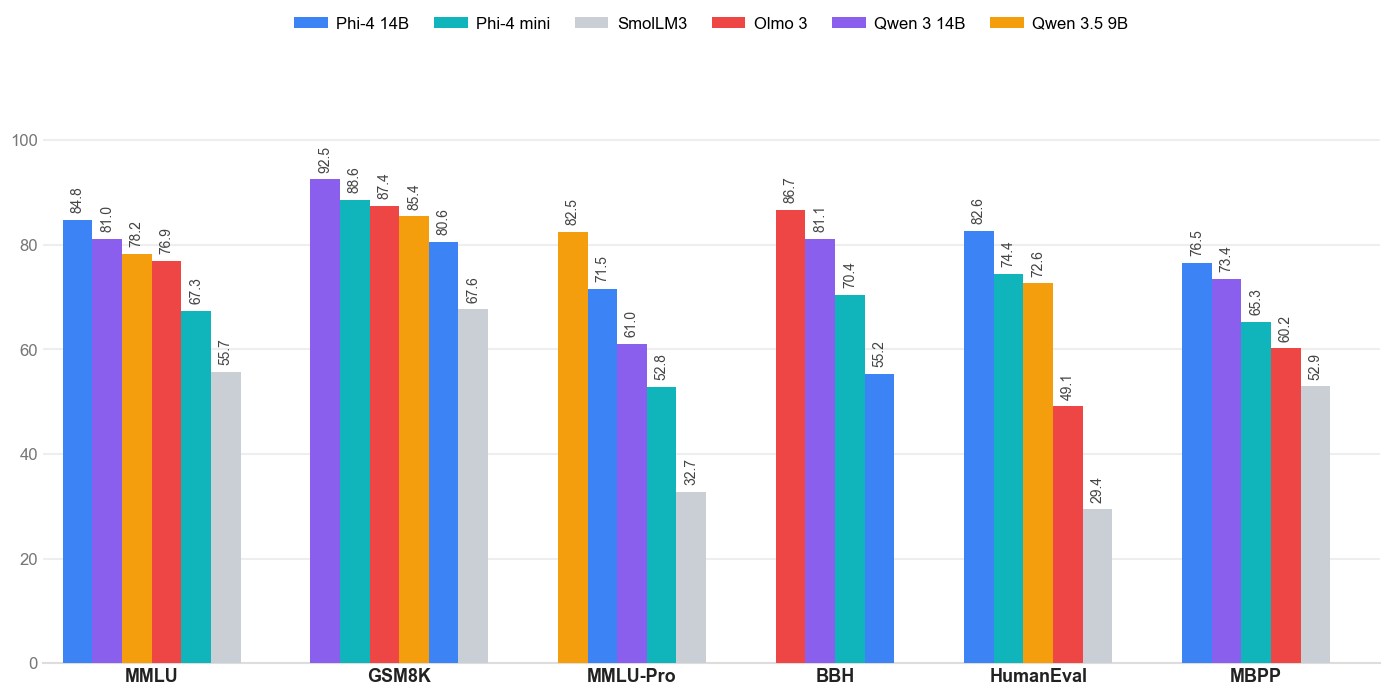
\includegraphics[width=0.95\textwidth]{figures/diag_bench_models.png}
      \caption{Scores détaillés par benchmark pour les principaux modèles $\le$ 14B paramètres.}
    \end{figure}
  \end{block}


  \begin{block}{Résultats}
    \begin{center}
    \small
    \begin{tabular}{lcccccc}
      \toprule
      \textbf{Modèle} & \textbf{MMLU} & \textbf{GSM8K} & \textbf{MMLU-Pro} & \textbf{BBH} & \textbf{HumanEval} & \textbf{MBPP} \\
      \midrule
      Phi-4 14B      & \textbf{84.8} & 80.6          & 71.5             & 55.2         & \textbf{82.6}     & \textbf{76} \\
      Phi-4 mini     & 67.3          & 88.6          & 52.8             & 70.4         & 74.4              & 65 \\
      SmolLM3 3B     & 55.7          & 67.6          & 32.7             & —            & 29.4              & 52 \\
      Olmo 3         & 76.9          & 87.4          & —                & \textbf{86.7}& 49.1              & 60 \\
      Qwen 3 14B     & 81.1          & \textbf{92.5} & 61.0             & 81.1         & —                 & 73 \\
      Qwen 3.5 9B    & 78.2          & 85.4          & \textbf{82.5}    & —            & 72.6              & — \\
      \bottomrule
    \end{tabular}
    \end{center}
    \vspace{0.5em}
    \textbf{Phi-4 14B} s'impose par sa régularité toutes tâches confondues. \textbf{Qwen 3.5 9B} surprend en dominant MMLU-Pro malgré ses 9B paramètres, surclassant des modèles plus massifs grâce à son architecture hybride.
  \end{block}


  \begin{block}{Efficacité Paramétrique}
    \begin{figure}
      \centering
      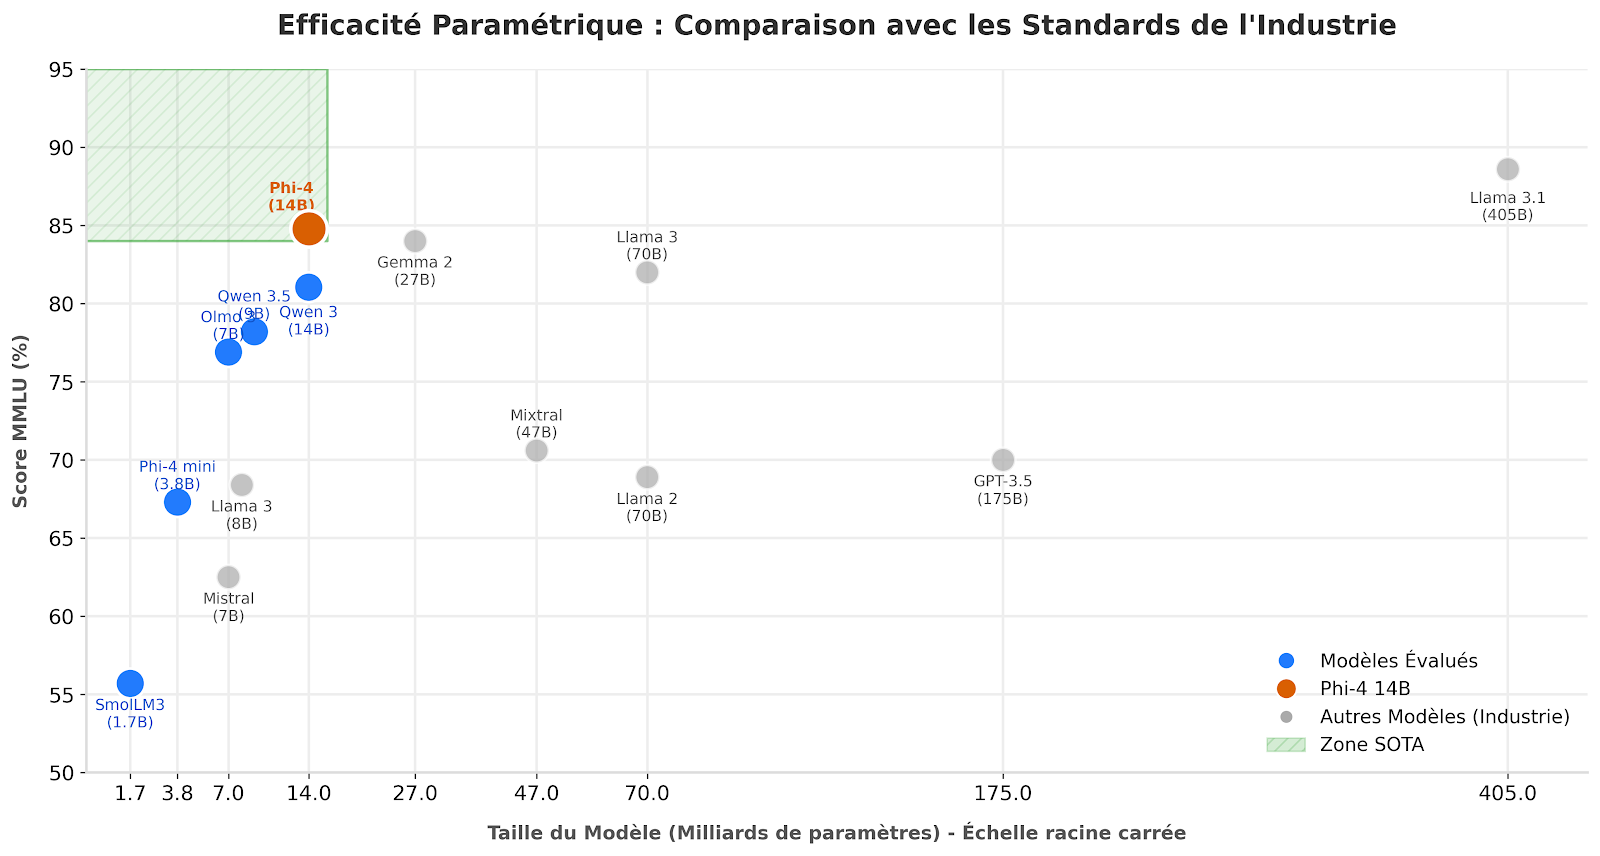
\includegraphics[width=0.95\textwidth]{figures/diagrame_perfmances_parametres.png}
      \caption{Efficacité Paramétrique : Comparaison avec les Standards de l'Industrie.}
    \end{figure}
  \end{block}


\end{column}

\separatorcolumn

% ====================
% COLONNE 3 — Applications et conclusions
% ====================
\begin{column}{\colwidth}

    \begin{figure}
      \centering
      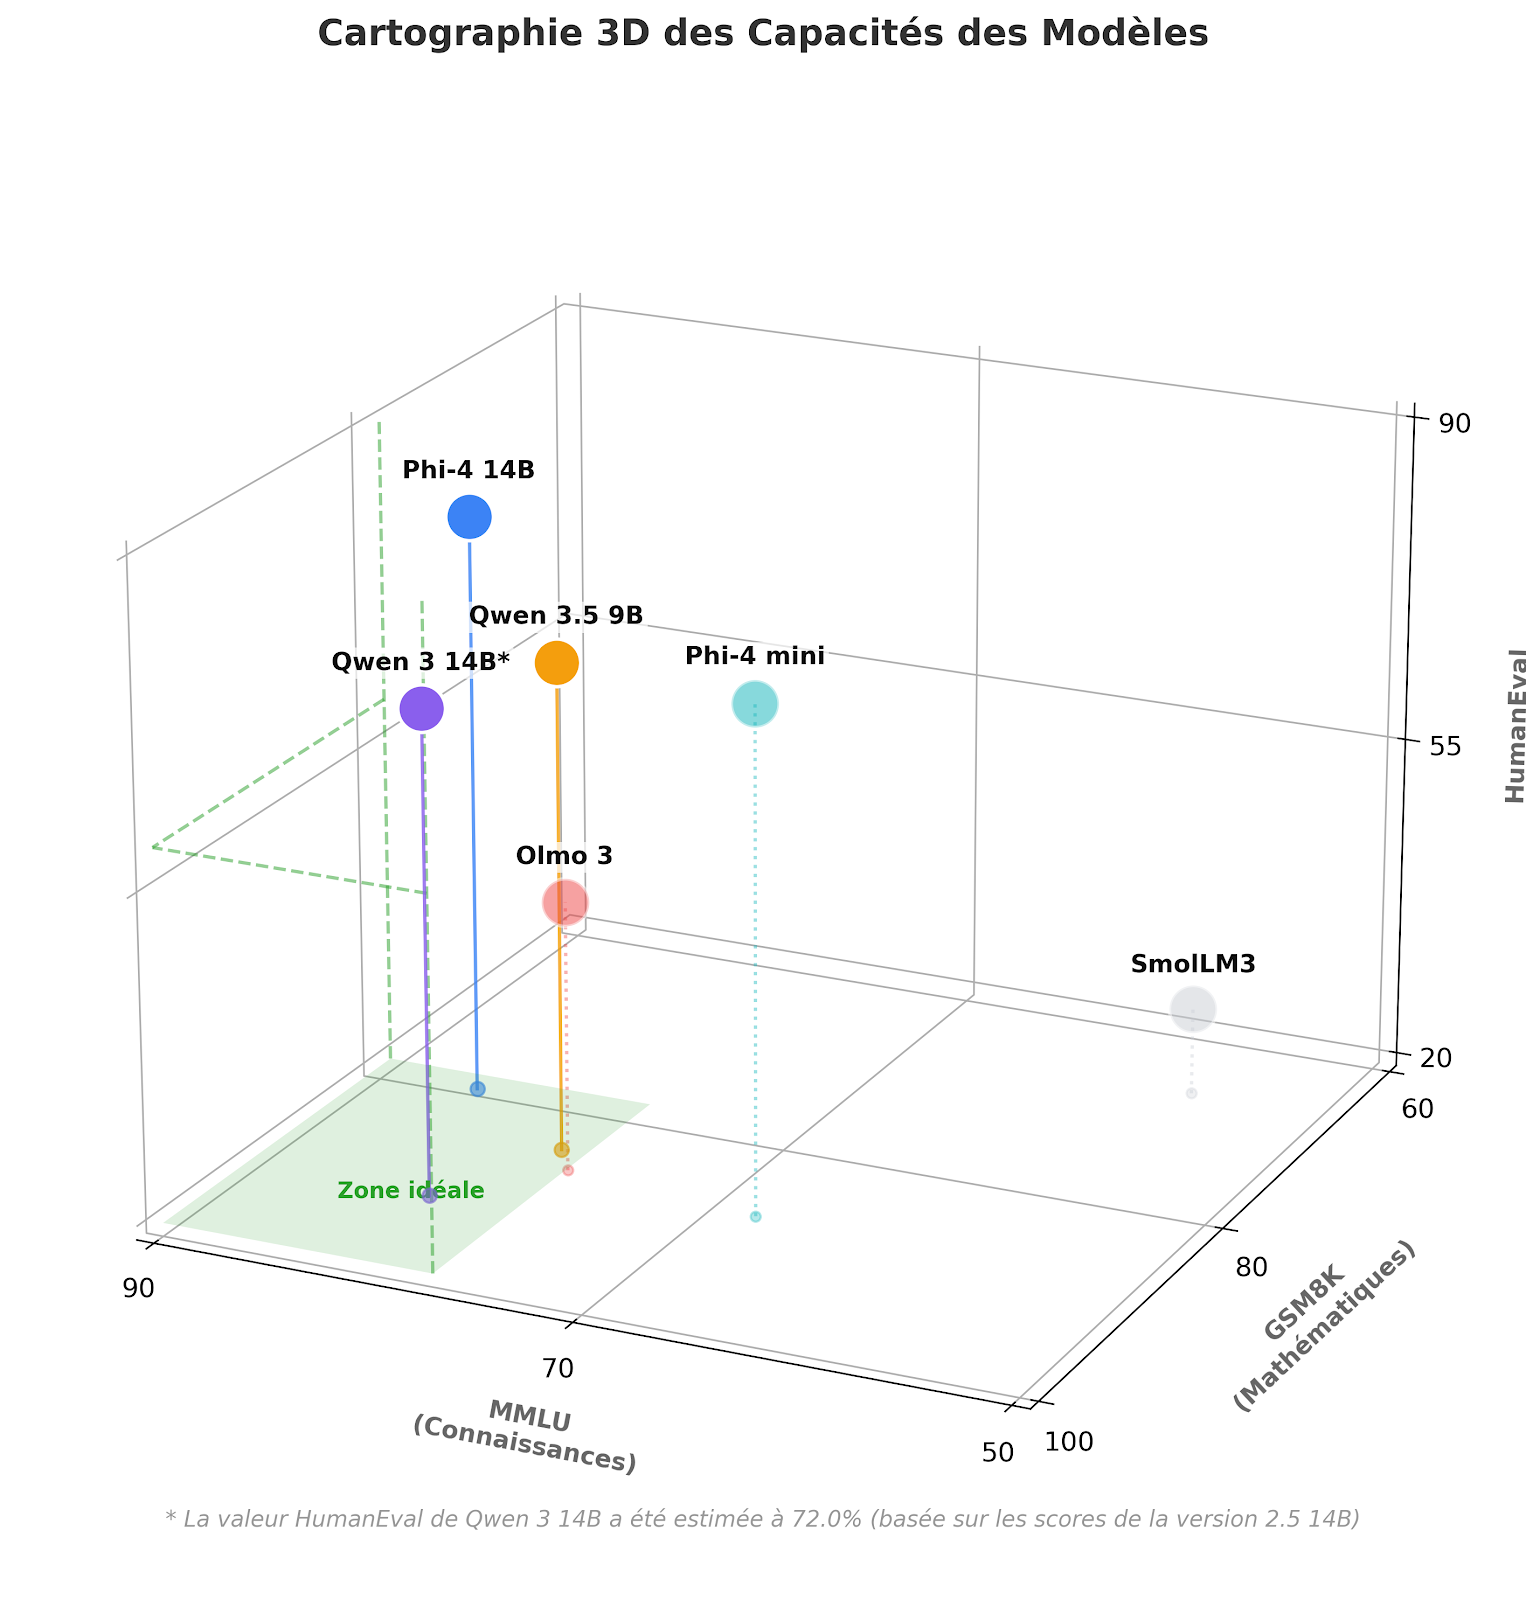
\includegraphics[width=0.85\textwidth]{figures/3D_representation.png}
      \caption{Représentation 3D des modèles SLM actuels.}
    \end{figure}

  \begin{block}{Défis Restants}
    Malgré leurs succès, les SLMs font face à plusieurs limitations :
    \begin{itemize}
      \item \textbf{Connaissances factuelles limitées :} La taille réduite limite la mémorisation encyclopédique, pallié par RAG.
      \item \textbf{Hallucinations :} Tendance persistante à générer des informations incorrectes sur des requêtes complexes.
      \item \textbf{Opacité des évaluations :} Protocoles hétérogènes (température, few-shot vs zero-shot) et évaluations souvent réalisées par les concepteurs eux-mêmes.
    \end{itemize}
  \end{block}

  \begin{exampleblock}{IA Embarquée et Edge Computing}
    L'un des principaux atouts des SLMs est leur capacité à fonctionner \textbf{localement}, sur des appareils aux ressources limitées (smartphones, PC portables, IoT).

    \textbf{Atouts} : Confidentialité, faible latence et fonctionnement hors-ligne sont garantis. Le RAG pallie le déficit de mémorisation. Empreinte carbone réduite de \textbf{60\%} : $\sim$\textbf{417} vs $\sim$\textbf{1015 tCO$_2$eq} pour un LLM comparable. Llama-2-7B est le modèle le plus énergétiquement efficace parmi les SLMs étudiés
  \end{exampleblock}

  \begin{alertblock}{Conclusion}
    Les SLMs ne sont pas de simples versions réduites des LLMs : ce sont des modèles efficaces et hautement optimisés. Notre étude désigne \textbf{Phi-4 14B} comme référence polyvalente, tandis que \textbf{Qwen 3.5 9B} démontre qu'un modèle plus petit peut surpasser des modèles plus grands sur les tâches analytiques.
  \end{alertblock}

  \begin{block}{Références}
    \bibliography{references_finales}
    \footnotesize{\bibliographystyle{plain}\bibliography{poster}}
  \end{block}

\end{column}

\separatorcolumn
\end{columns}
\end{frame}

\end{document}
